\documentclass[11p]{article}
% Packages
\usepackage{amsmath}
\usepackage{graphicx}
\usepackage[swedish]{babel}
\usepackage[
    backend=biber,
    style=authoryear-ibid,
    sorting=ynt
]{biblatex}
\usepackage[utf8]{inputenc}
\usepackage[T1]{fontenc}
%Källor
\addbibresource{mall.bib}
\graphicspath{ {./images/} }

\title{Labrapprt \\ \small Fysik 1}
\author{Magnus Silverdal }
\date{\today}

\begin{document}

    \begin{titlepage}
        \begin{center}
            \vspace*{1cm}

            \Huge
            \textbf{Laboration 5}

            \vspace{0.5cm}
            \LARGE
            Ellära

            \vspace{1.5cm}

            \textbf{Gabriel Nilsson Högberg}

            \vfill


            Fysik 1

            \vspace{0.8cm}

            
\includegraphics[width=0.4\textwidth]{../images/NTI Gymnasiet_Symbol_print_svart.png}

            \Large
            Teknikprogrammet\\
            NTI Gymnasiet\\
            Umeå\\
            \today

        \end{center}
    \end{titlepage}
    \section{Syfte och frågeställning}
    \section{Del 1}
    Vi mätte strömmen som gick genom kretsen genom att sätta dit multimetern och därefter fick vi det till 0,08A (Se bild nedan).
    Efter det hade vi ett batteri med 9 volt och för att räkna ut resistansen tog vi spänning delat med strömmen.
    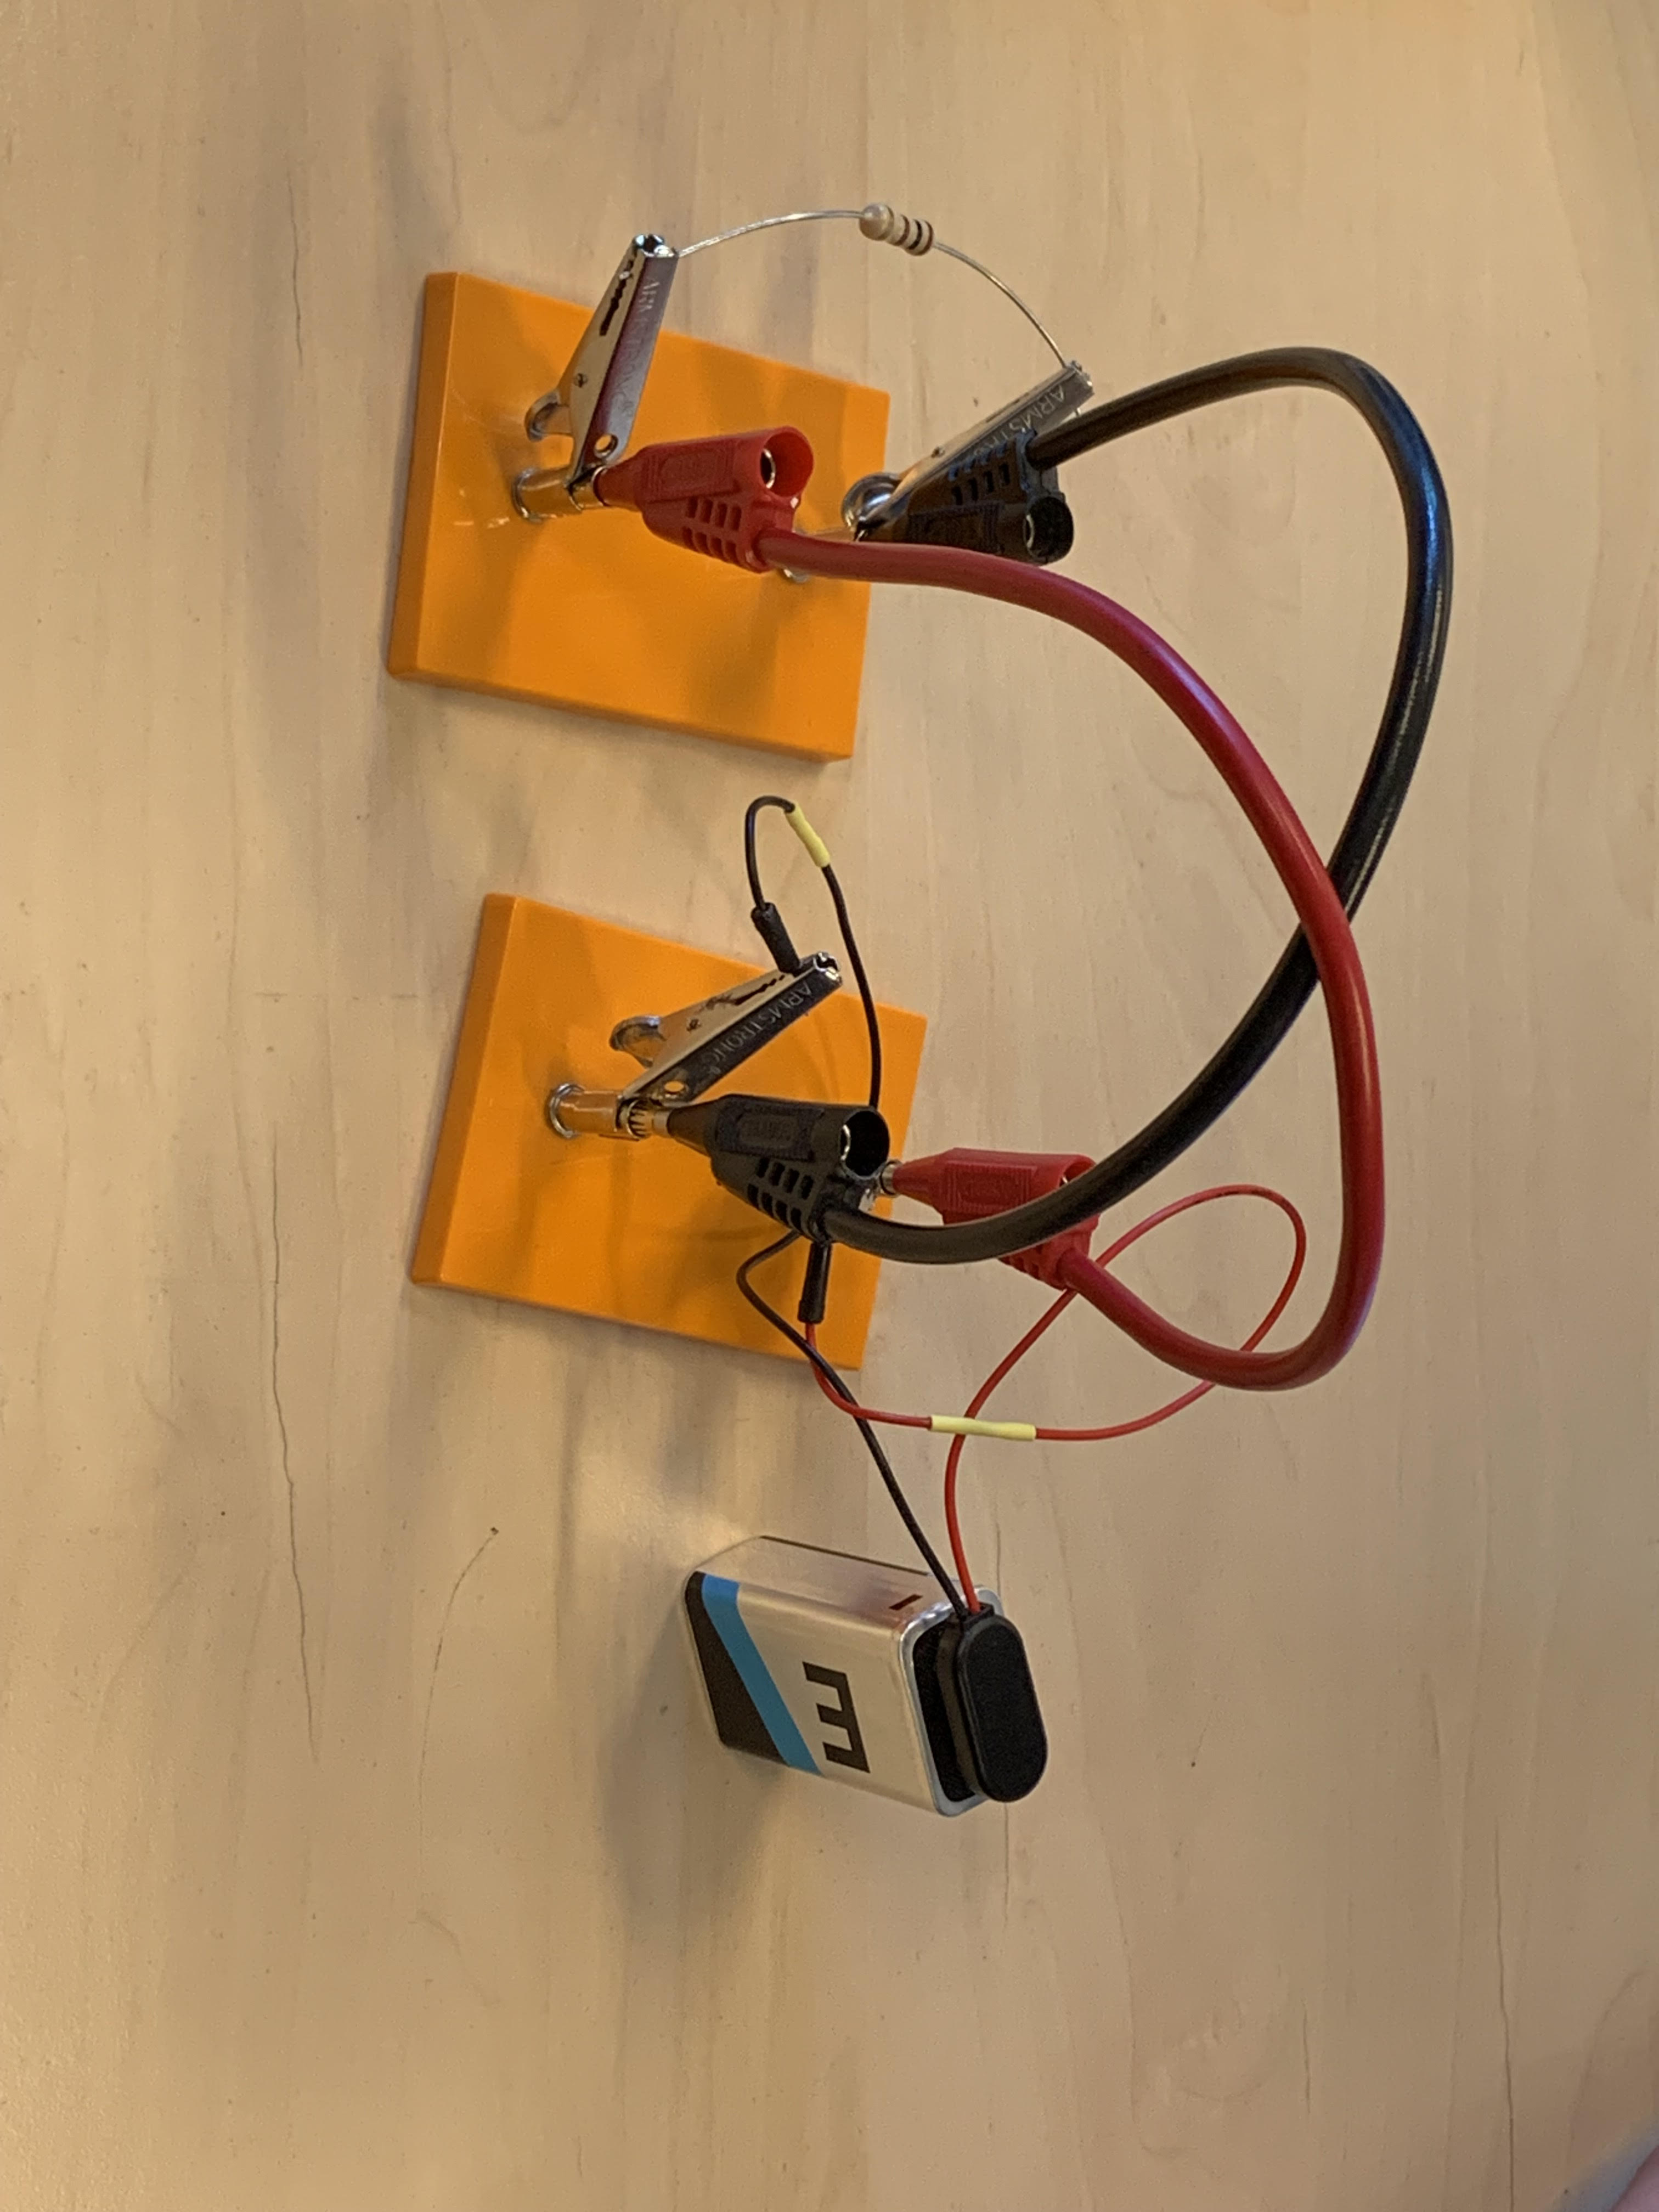
\includegraphics[width=0.4\textwidth]{../images/BildDel1}
    \subsection{Material och metod}
    \begin{itemize}
        \item 9 Volt Batteri
        \item 1 Multimeter
        \item två kablar
        \item tre kopplingssplintar
        \item två krokodilklämmor
        \item två motstånd
    \end{itemize}

    Metoden var att göra en enkel koppling med en resistans kopplad med ett batteri och sedan mäta strömmen med multimetern för att räkna ut resistansen efteråt.
    \subsection{Resultat}
    Våra resultat var att strömmen var 0,08A, spänningen var 9 volt och resistansen var 112,5 ohm.
    \subsection{Analys}
    För att räkna ut resistansen använde vi formeln \begin{equation} R = \frac{9}{0,08} \end{equation} med detta satte vi in våran spänning(U) och våran ström(I) och därefter fick vi ut 112,5 ohm
    \section{Del 2}
    vi mätte strömmen som gick genom kretsen för att se strömmen efter den gått genom resistansen och spänningen som var över ena resistansen som var seriekopplad med en annan (se bild nedan).
    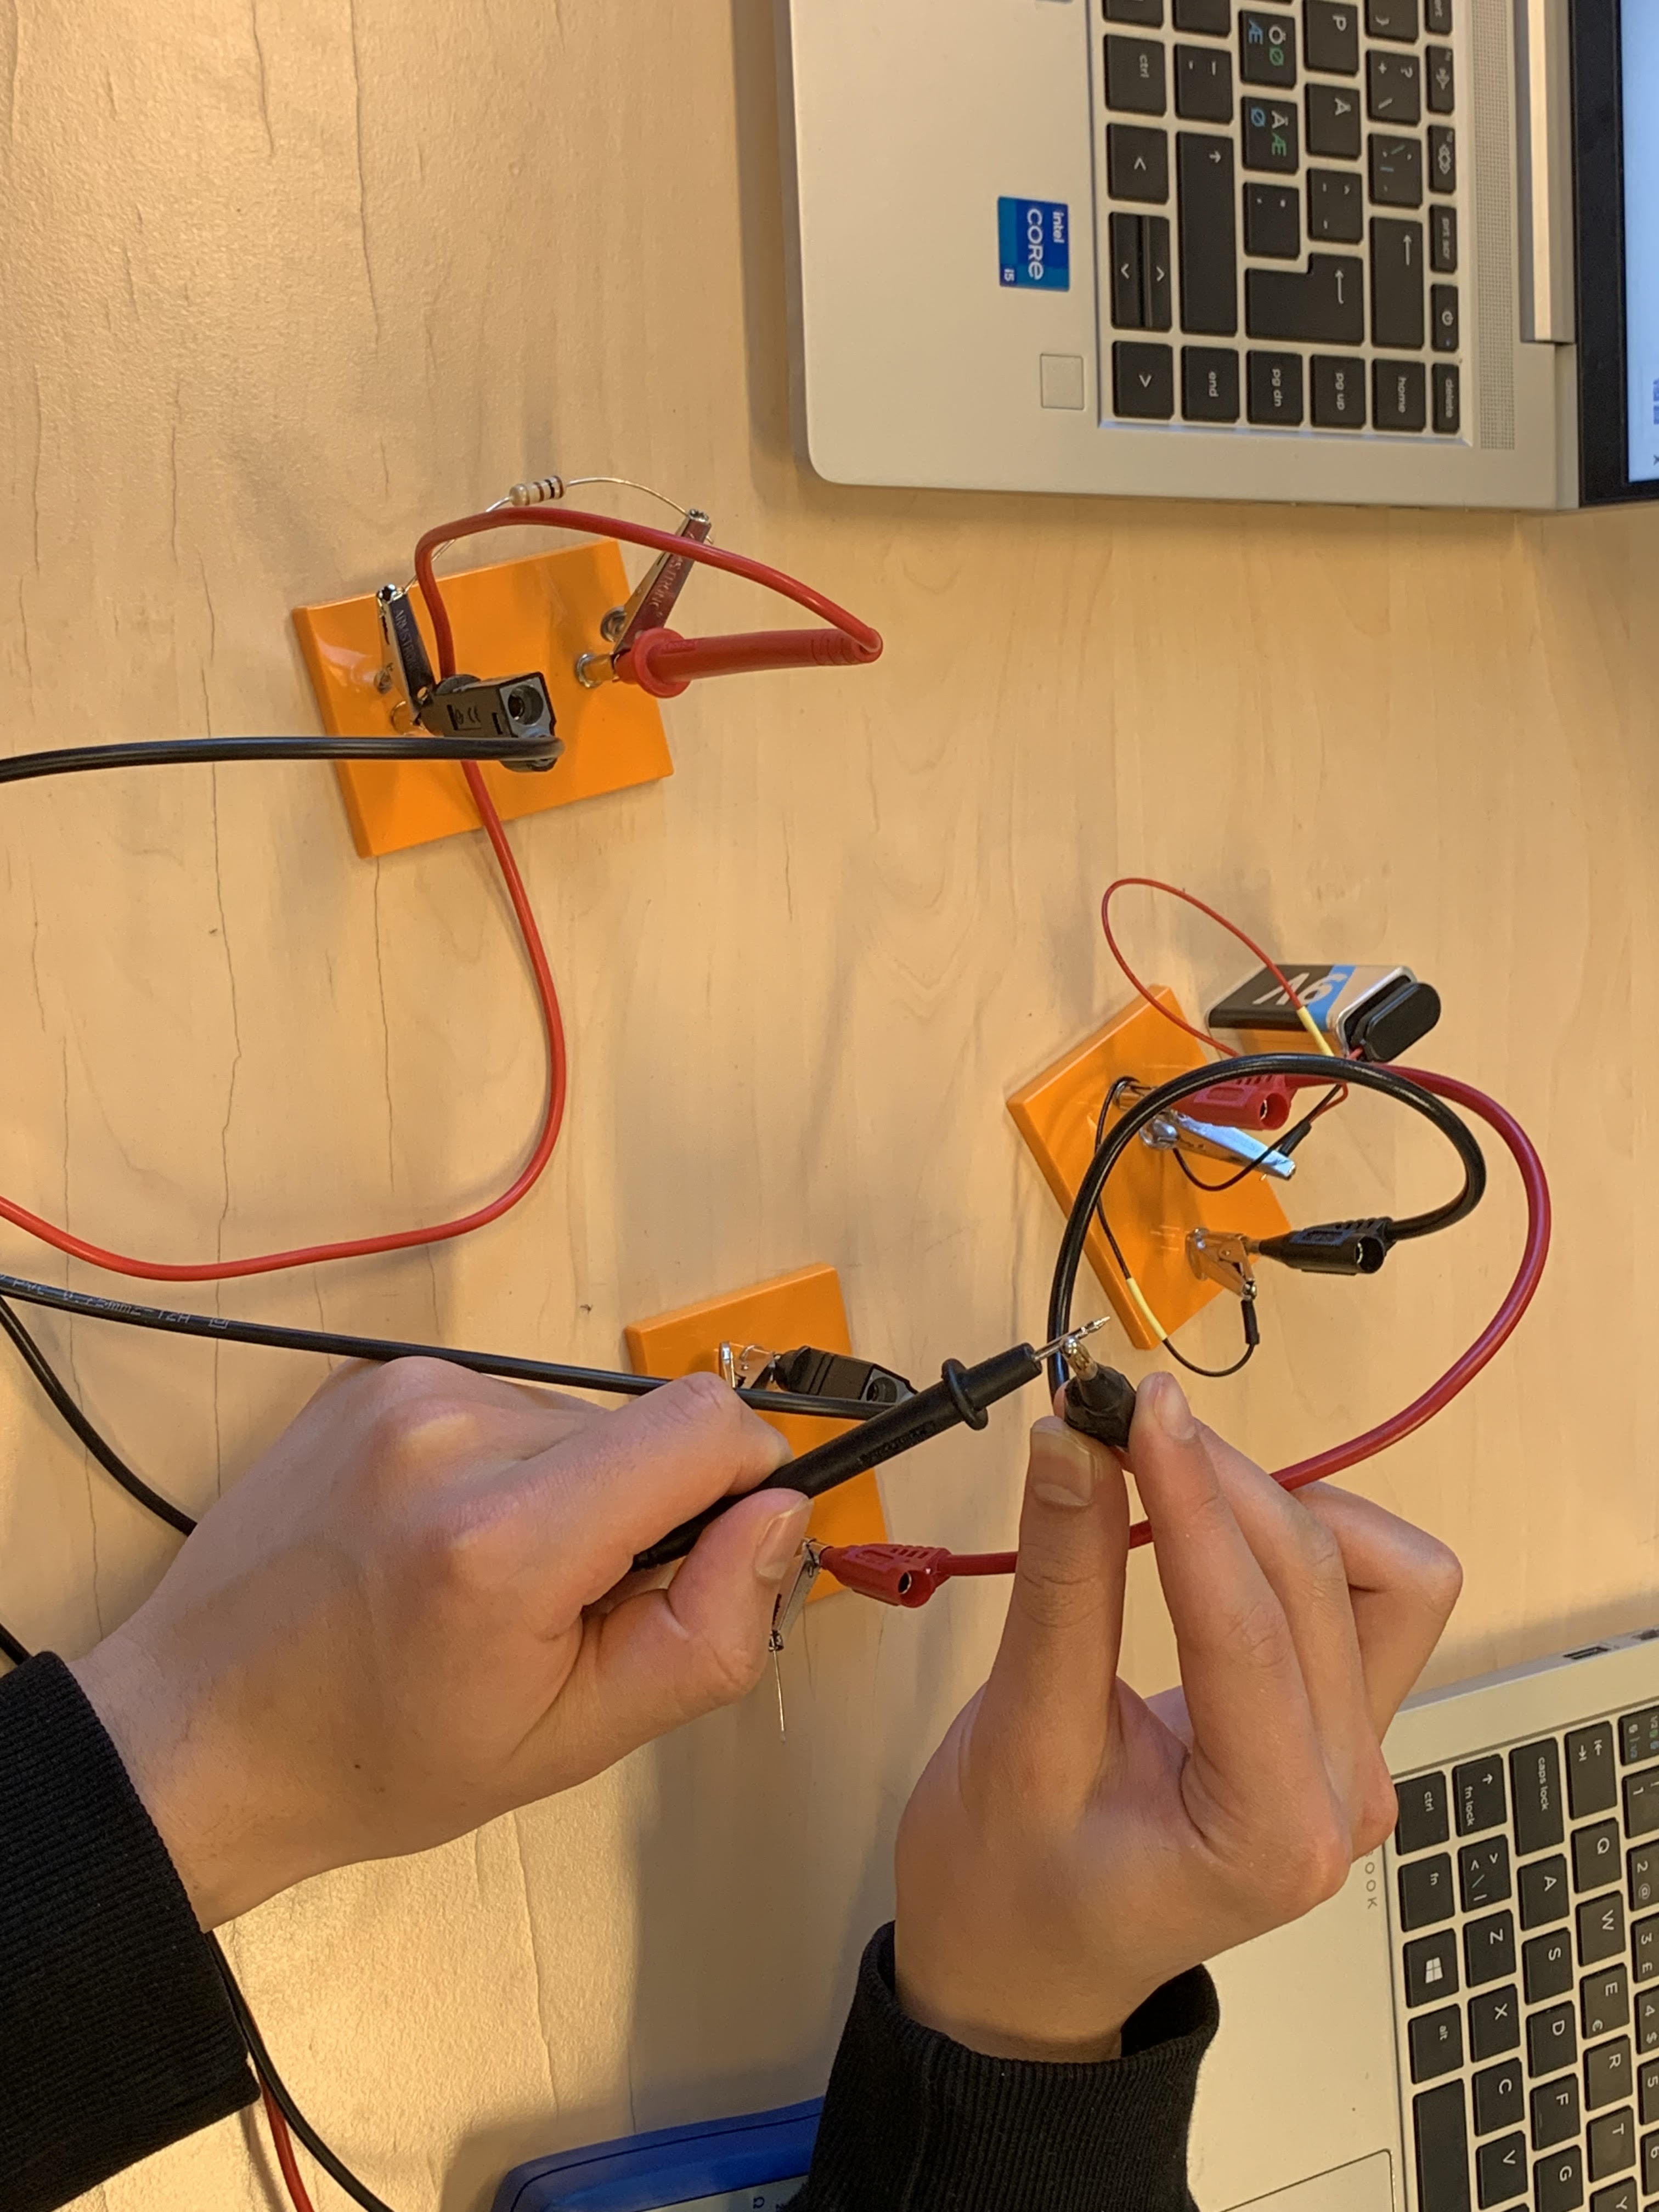
\includegraphics[width=0.4\textwidth]{../images/BildDel2}
    \subsection{Material och metod}
    \begin{itemize}
        \item 9 Volt Batteri
        \item 1 Multimeter
        \item två kablar
        \item tre kopplingssplintar
        \item två krokodilklämmor
        \item två motstånd
    \end{itemize}

    Metoden var att seriekoppla två resistanser till ett bateri och sedan mäta ström och spänning med multimetern
    \subsection{Resultat}
    Spänningen över ena resistansen är 4,05 volt och strömmen är 0,04A
    \subsection{Analys}
    Enligt teorin borde vi fått spänningen 4,5 eftersom \begin{equation} U = 112,5 * 0,04 \end{equation} och för strömmen borde det varit 0,036A eftersom \begin{equation} I = \frac{4,05}{112,5} \end{equation}
    \section{Del 3}
    \subsection{Material och metod}
    \subsection{Resultat}
    \subsection{Analys}
    \section{Diskussion}
\end{document}
